% klasa report,jednostronny
\documentclass[a4paper, 11pt, oneside]{article}

% kodowanie
\usepackage[utf8]{inputenx}
\usepackage[T1]{fontenc}
\usepackage{listings}


% czcionka Arial
\usepackage{helvet}
\renewcommand{\familydefault}{\sfdefault}

% jezyk tekstu
%\usepackage{polski}
%\usepackage[polish]{babel}

% marginesy
\usepackage[inner=30mm,outer=20mm,top=25mm,bottom=25mm]{geometry}

% interlinia
\linespread{1.15}

% paczka do zarzadza headerami i footerami; ustawienie numeracji w dolnym zewnetrznym rogu
\usepackage{fancyhdr}   
\pagestyle{fancy}
\fancyhead{}% clear headers
\fancyfoot{}% clear footers
\renewcommand{\headrulewidth}{0pt}% eliminate horizontal line
\fancyfoot[RO, LE]{\thepage}
% redefinicja stylu plain (zeby na stronach z tytulem rozdzialu tez bylo dobrze
\fancypagestyle{plain}{%
  \fancyhf{}%
  \fancyfoot[RO, LE]{\thepage}%
  \renewcommand{\headrulewidth}{0pt}% Line at the header invisible
  \renewcommand{\footrulewidth}{0pt}% Line at the footer visible
}

% Akapit do wyboru:

% wcięcie 5mm
% \usepackage{indentfirst}
% \setlength{\parindent}{5mm}
% \setlength{\parskip}{0ex} 

% odstep 4 pomiedzy akapitami
 \setlength{\parindent}{0mm}
 \setlength{\parskip}{2ex} 


% paczka do rysunkow
\usepackage{graphicx}
\usepackage{float}
% foldery z rysunkami
\graphicspath{ {Rysunki/} {Wykresy/} }
% domyslnie numeracja wg rozdzialow
% ponizej ciagla w pracy
% \usepackage{chngcntr}
% \counterwithout{figure}{chapter}

%ponizej zeby podpisy mialy dobry rozmiar i byly gdzie trzeba w rysunkach
\usepackage{caption}
\DeclareCaptionFormat{myformat}{\fontsize{9}{10}\selectfont#1#2#3}
\captionsetup{format=myformat}
\captionsetup[figure]{slc=off}

% paczki do robienia ladnych tabel, ustawienie podpisow itd, zmiana tablica na tabela
\usepackage{booktabs}
\usepackage[svgnames,table]{xcolor}
\usepackage{threeparttable}
\captionsetup[table]{justification=justified,singlelinecheck=false}
\usepackage{pifont}

%\renewcommand{\tablename}{Tabela}

% zmiana czcionek w (pod)rozdziałach
\usepackage{anyfontsize}
\usepackage{titlesec}
\titleformat{\chapter}[display]
  {\normalfont\sffamily\fontsize{14}{15}\selectfont\bfseries\color{black}}
  {\chaptertitlename\ \thechapter}{14pt}{\fontsize{14}{15}\selectfont}
\titleformat{\section}
  {\normalfont\sffamily\fontsize{13}{14}\selectfont\bfseries\color{black}}
  {\thesection}{13pt}{}
\titleformat{\subsection}
  {\normalfont\sffamily\fontsize{12}{13}\selectfont\bfseries\color{black}}
  {\thesubsection}{12pt}{}
\titlespacing\chapter{0pt}{0pt plus 4pt minus 2pt}{12pt plus 2pt minus 2pt}
\titlespacing\section{0pt}{6pt plus 4pt minus 2pt}{0pt plus 2pt minus 2pt}
\titlespacing\subsection{0pt}{0pt plus 4pt minus 2pt}{0pt plus 2pt minus 2pt}

% zalaczanie stron pdf
\usepackage{pdfpages}

% generowanie tekstu- do wyrzucenia
\usepackage{lipsum}
%biblioteka matematyczna
\usepackage{ amsmath}
%tikz
\usepackage{pgfplots} 

%Bibliotek do pisania pseudo kodu i kodu
\usepackage{amsmath}
\usepackage{algorithm}
\usepackage[noend]{algpseudocode}

% and optionally (as of Pgfplots 1.3): 
\pgfplotsset{compat=newest} 
\pgfplotsset{plot coordinates/math parser=false} 
\newlength\figureheight 
\newlength\figurewidth

\setcounter{MaxMatrixCols}{20} 


%bibliografia
\usepackage[backend=biber]{biblatex}
\addbibresource{bibs.bib}

%strona tytułowa
\title{%
  SST MISK \\Projekt semestralny \\
  \vspace{5mm}
  \large Monitorowanie celu za pomocą autonomicznej chmury dronów\\
  opracowanie algorytmu kooperacji i symulacja}
\author{Jerzy Baranowski\\Artur Czopor\\Ignacy Ruksza \\Krzysztof Zarzycki }

\date{\today}

\begin{document}

\maketitle
\newpage
\section{Opis projektu}
Celem projektu jest stworzenie i symulacja działania algorytmu sterowania rojem dronów tak by w sposób optymalny formowały ustaloną formację nad wyznaczonym celem. 
\section{Użyte oprogramowanie}

Symulacja wyżej opisanego zadania została wykonana w programie symulacyjnym V-Rep połączonym dedykowanym API ze środowiskiem Matlab. W celu realizacji zadania został zaimplementowany w języku M skrypt optymalizujący trasę przelotu drona w zależności od pozycji celu i roju.  Obiekty latający odwzorowane są w środowisku V-Rep poprzez model symulacyjny “Quadricopter”, który posiada możliwość sterowania poprzez wyznaczenia pozycji docelowej. Model ten został dostarczony przez producenta oprogramowania i ingerencja w jego mechanikę nie jest celem projektu. W celu obejścia ograniczeń modelu trajektoria wyliczana jest wyznaczana poprzez generację punktów docelowych dla kolejnych chwil dla każdego z dronów.

\begin{figure}[H]
\centering
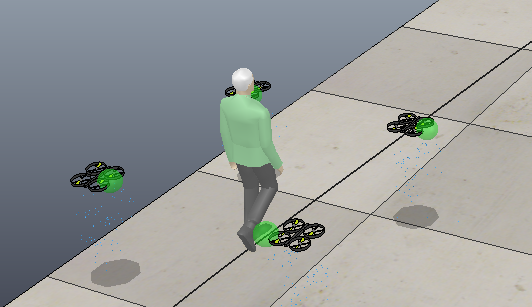
\includegraphics[scale=0.5]{simulation1.png}
\caption{Przykładowa scena z symulatora V-Rep.}

\end{figure}

\section{Opis algorytmu}
Pętla główna programu obliczającego trajektorię dronów zaprezentowana jest na poniższym diagramie akcji
\section{Implementacja}
\begin{figure}[H]
\centering
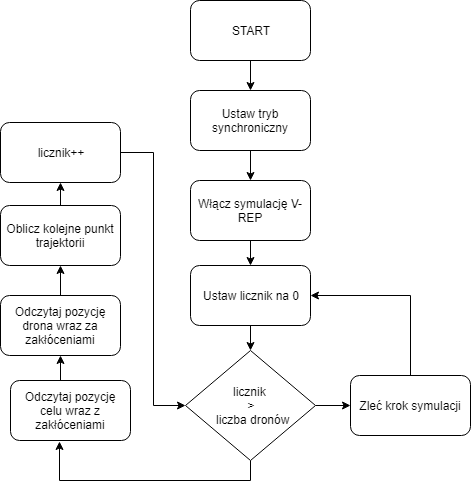
\includegraphics[scale=0.5]{uproszczony_digram_akcji.png}
\caption{Uproszczony diagram akcji.}

\end{figure}
\section{Wynik działania}
\section{Wnioski}
\end{document}